\section{模型构建与结构优化}
\par{本章通过 Materials Studio 8.0 中的Materials Visualizer模块来构建丁酸甲酯、丁烯酸甲酯、油酸甲酯、反油酸甲酯、正己烷等吸附分子和H-ZSM-5微介孔分子筛的模型。使用 Dmol3模块,采用量子力学的方法优化丁酸甲酯、丁烯酸甲酯、油酸甲酯、反油酸甲酯和正己烷等吸附分子模型结构并对其赋予ESP电荷。使用Forcite模块,采用分子力学的方法优化构建的微介孔H-ZSM-5分子筛模型,并将结构优化后的H-ZSM-5分子筛的XRD与标准谱图进行对比,验证模型的正确性。}
\subsection{吸附分子模型构建与优化}
\subsubsection{Dmol3参数设置}\label{Dmol3参数设置}
\par{本小节使用Dmol3模块对吸附分子进行结构优化以及确定原子ESP电荷,相关参数设置如下:}
\begin{enumerate}
    \item 任务选择:结构优化(Geometry Optimization),精度为Fine精度;
    \item 密度泛函(Functional)选择:广义梯度近似(mGGA-M06L),收敛判据选择Fine精度。能量、梯度和位移的收敛阈值分别为1.0×$10^{-5}$Ha、0.002Ha/Å和0.005Å,采用DIIS技术加速SCF收敛;
    \item 核处理(Core Treatment)选择:考虑所有电子(All Electron),数值基组选择默认的DNP,轨道截断精度为Fine精度;
    \item 性能选择:布局分析(Population analysis)。
\end{enumerate}
\par{与B3LYP泛函相比,mGGA-M06L是目前理论计算中使用的最新和最广的泛函,可以很好地描述弱相互作用,计算结果精度很高\cite{zhao2006new,zhao2011applications}。采用Dmol3 Analysis 的布局分析功能,对结构优化后的分子模型赋予ESP电荷。}
\subsubsection{吸附分子几何优化构象}
\par{使用Materials Visualizer模块搭建吸附分子模型,然后使用Dmol3模块,采用 \ref{Dmol3参数设置} 所设参数对吸附分子进行结构优化并赋予ESP电荷。赋予ESP电荷后的吸附分子的结构优化构象见\reffig{fig:build}。}

\begin{figure}[H]
    \centering

    \subfigure[丁酸甲酯(1.732Å×7.794Å×2.755 Å)]{
    \begin{minipage}[t]{0.5\linewidth}
    \centering
    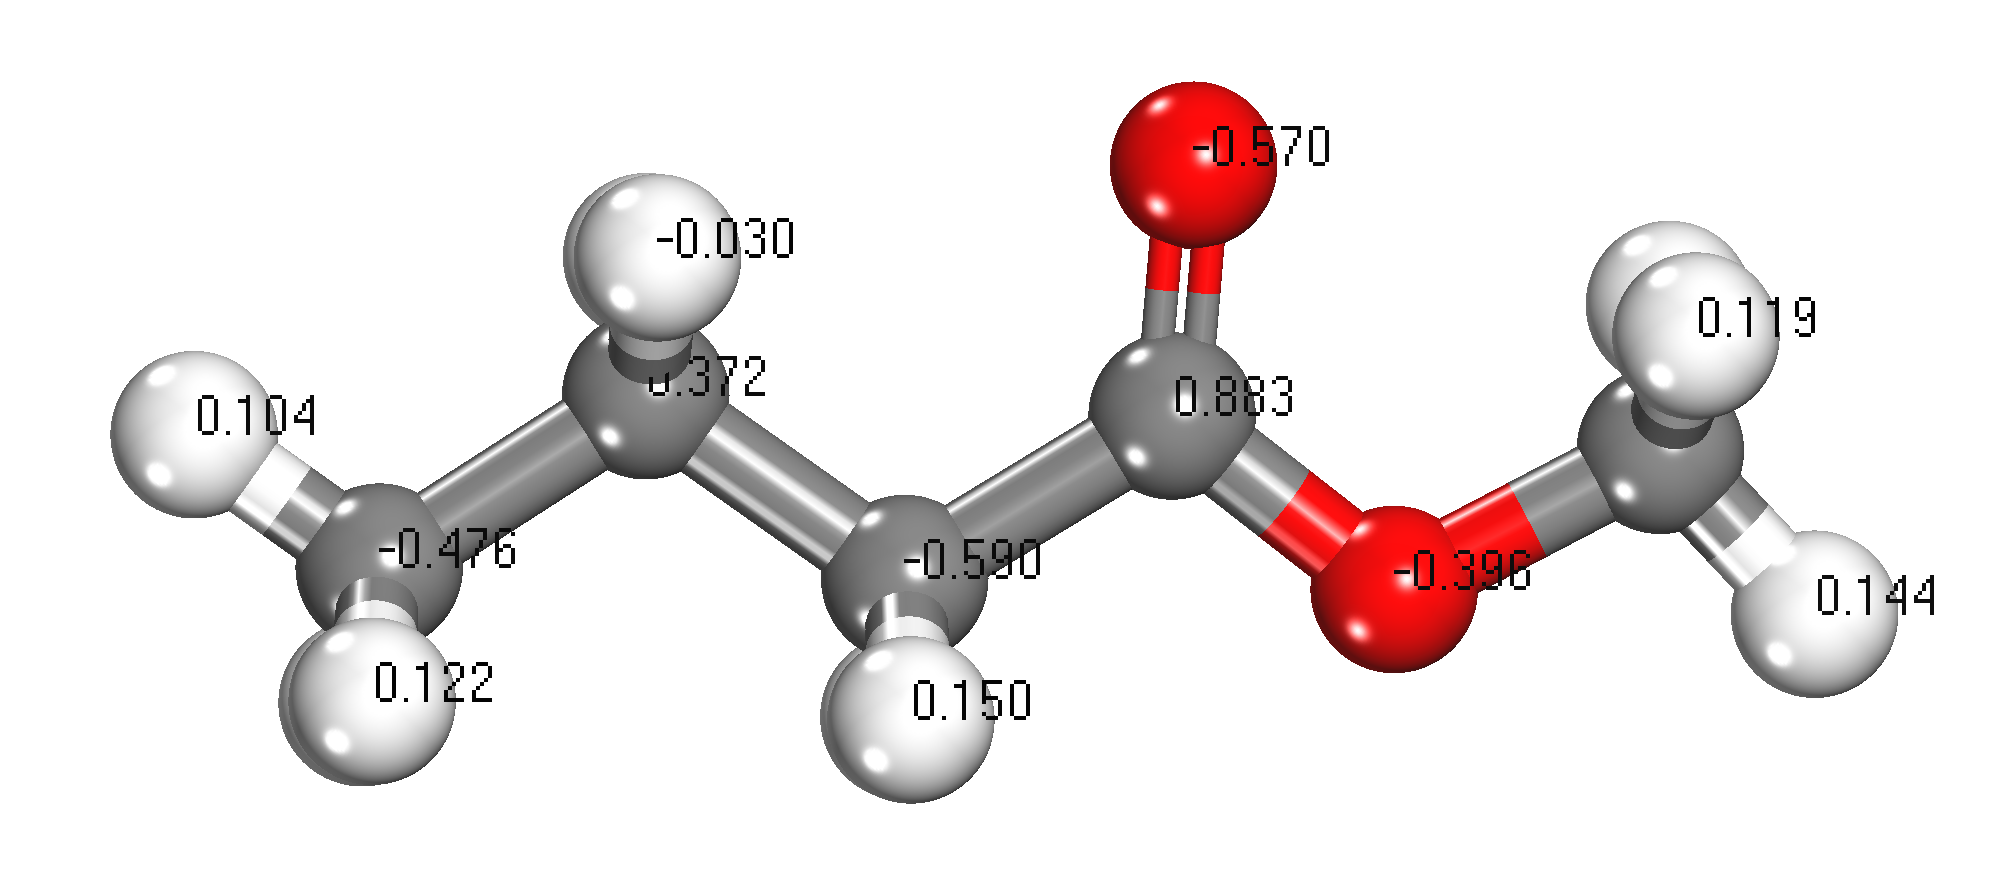
\includegraphics[width=3in]{figure/Building/saturatedC4.png}
    %\caption{fig1}
    \end{minipage}%
    }%
    \subfigure[丁烯酸甲酯(1.732Å×7.757Å×2.755 Å)]{
    \begin{minipage}[t]{0.5\linewidth}
    \centering
    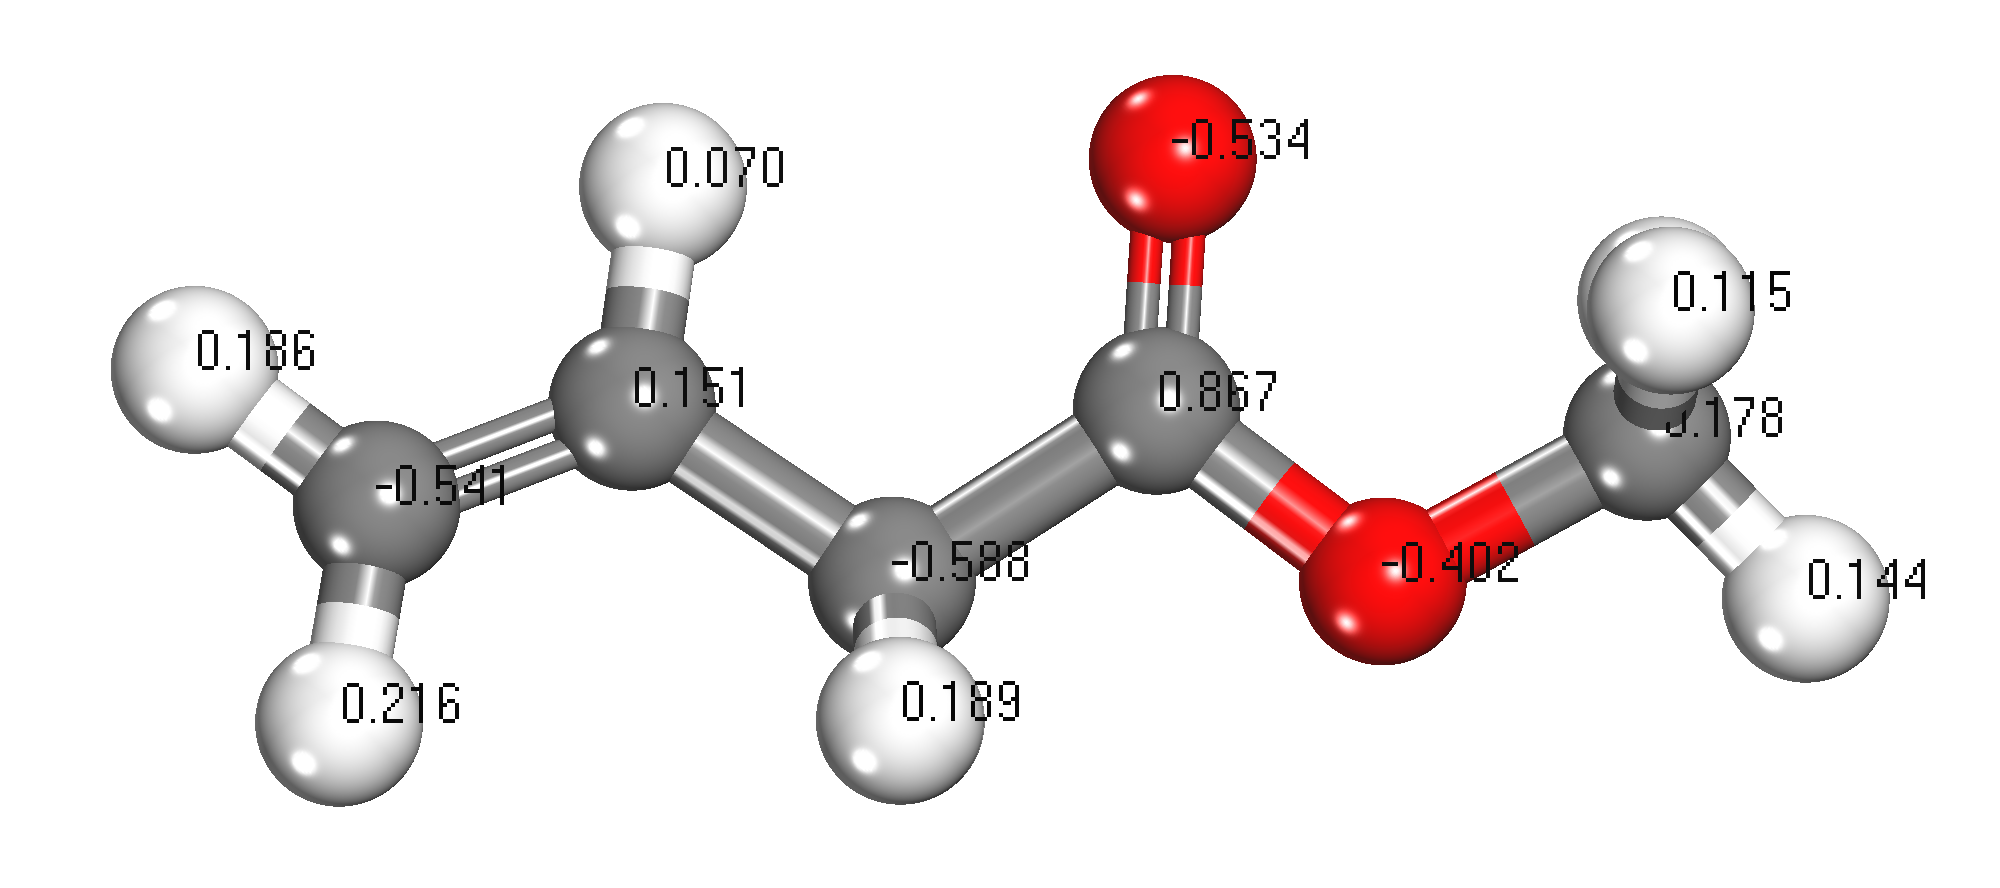
\includegraphics[width=3in]{figure/Building/unsaturatedC4.png}
    %\caption{fig2}
    \end{minipage}%
    }%

    \subfigure[油酸甲酯(2.879Å×25.220Å×2.967 Å)]{
    \begin{minipage}[c]{1\textwidth}
    \centering
    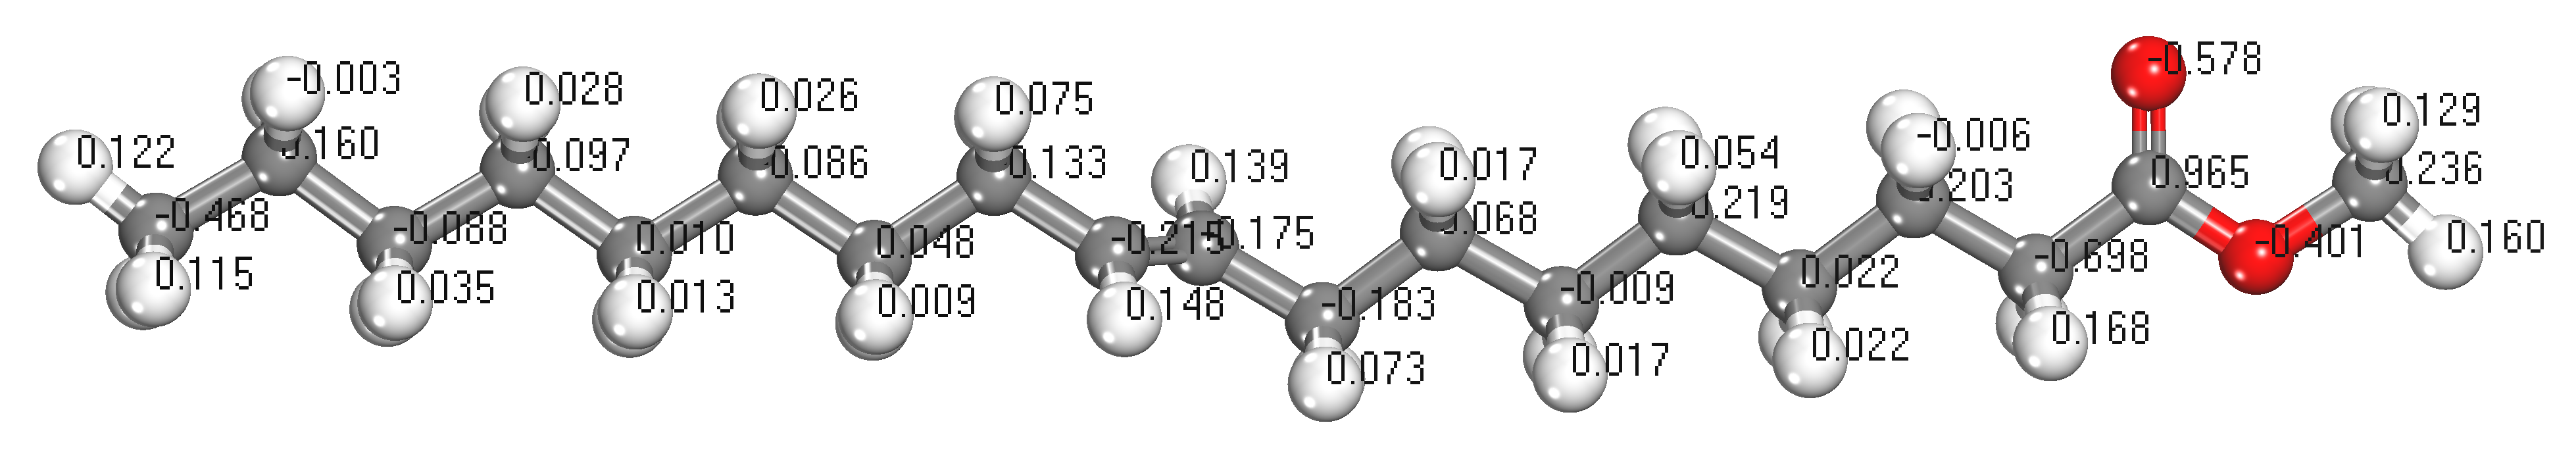
\includegraphics[width=6in]{figure/Building/C18-cis.png}
    %\caption{fig2}
    \end{minipage}%
    }%

    \subfigure[反油酸甲酯(2.879Å×24.579Å×3.017Å)]{
    \begin{minipage}[c]{1\textwidth}
    \centering
    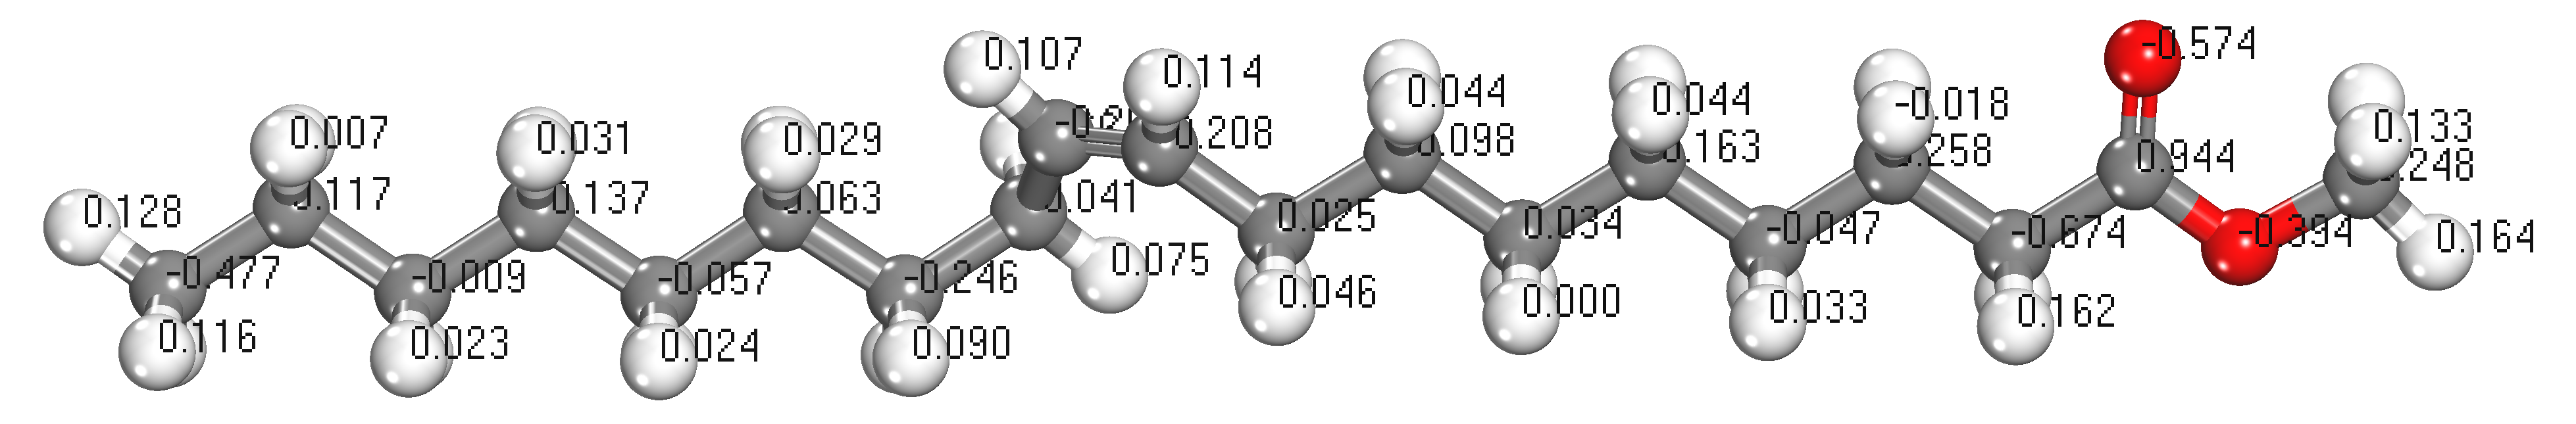
\includegraphics[width=6in]{figure/Building/C18-trans.png}
    %\caption{fig2}
    \end{minipage}%
    }%

    \subfigure[正己烷(1.732Å×8.141Å×2.511 Å)]{
    \begin{minipage}[t]{0.5\linewidth}
    \centering
    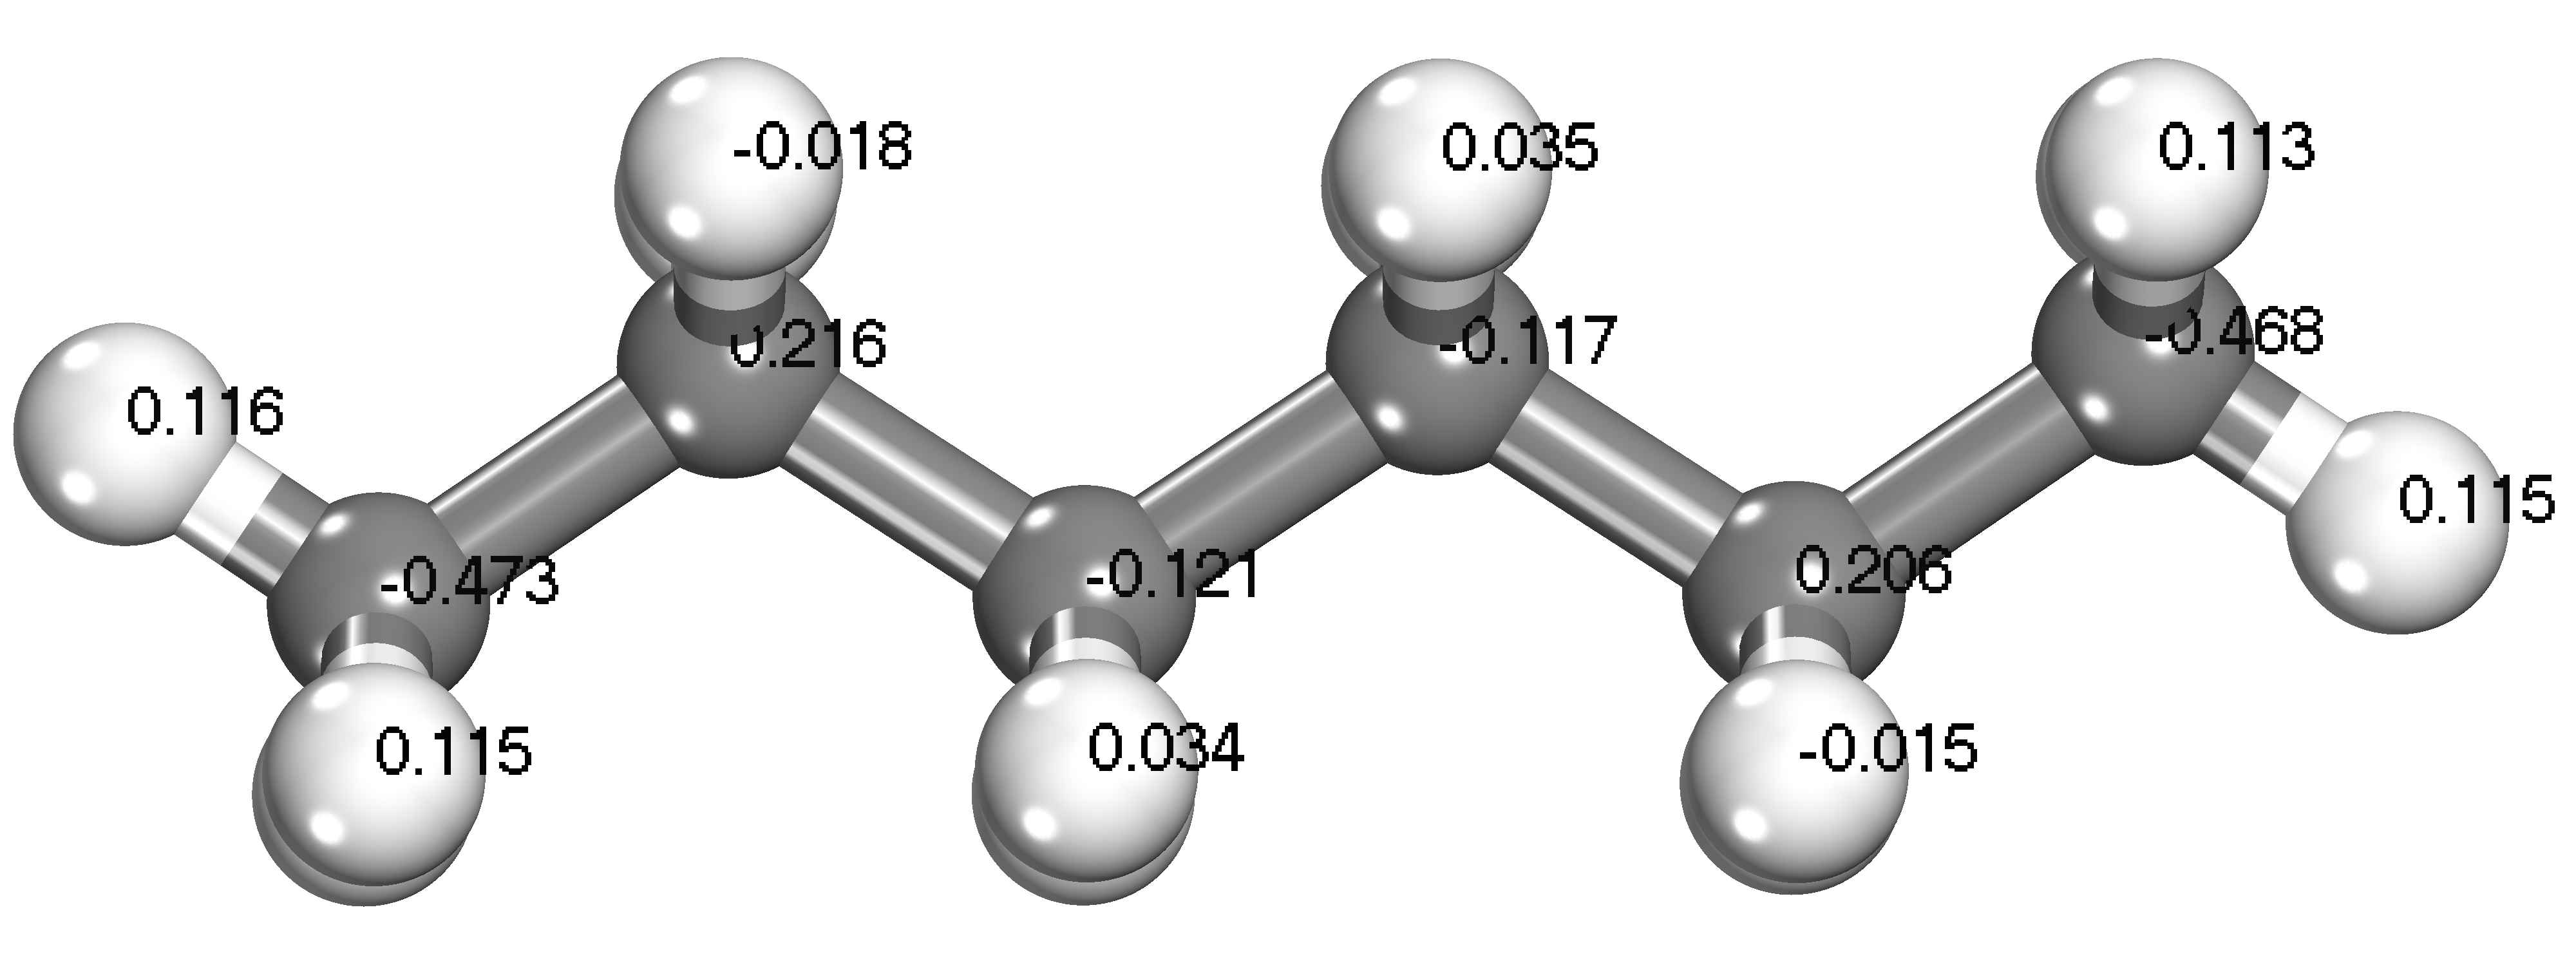
\includegraphics[width=3in]{figure/Building/C6.png}
    %\caption{fig2}
    \end{minipage}%
    }%
    \caption{吸附分子几何优化构象和ESP电荷图}
    \label{fig:build}
\end{figure}

% \subsubsection{丁酸甲酯模型结构}
% \par{本文通过使用Materialss Studio 8.0中Materialss Visualizer模块搭建丁酸甲酯模型,然后使用Dmol3模块对其设置上述参数,然藏对丁酸甲酯模型进行结构优化。优化后的丁酸甲酯分子模型的三维尺寸为1.732Å×7.794Å×2.755 Å,其具体三维结构见\reffig{fig:sC4ESP}。H-ZSM-5分子筛的正弦孔道孔径为5.5Å×5.1Å,直孔道孔径为5.3Å×5.6Å\cite{baerlocher2007atlas},故丁酸甲酯分子可以通过H-ZSM-5分子筛的孔道。将优化后的丁酸甲酯模型用Dmol3 Analysis赋予ESP电荷,其电荷分布见\reffig{fig:sC4ESP},其中C原子为灰色,H原子为白色,O原子为红色。}
% \begin{figure}[H]
%     \centering
%     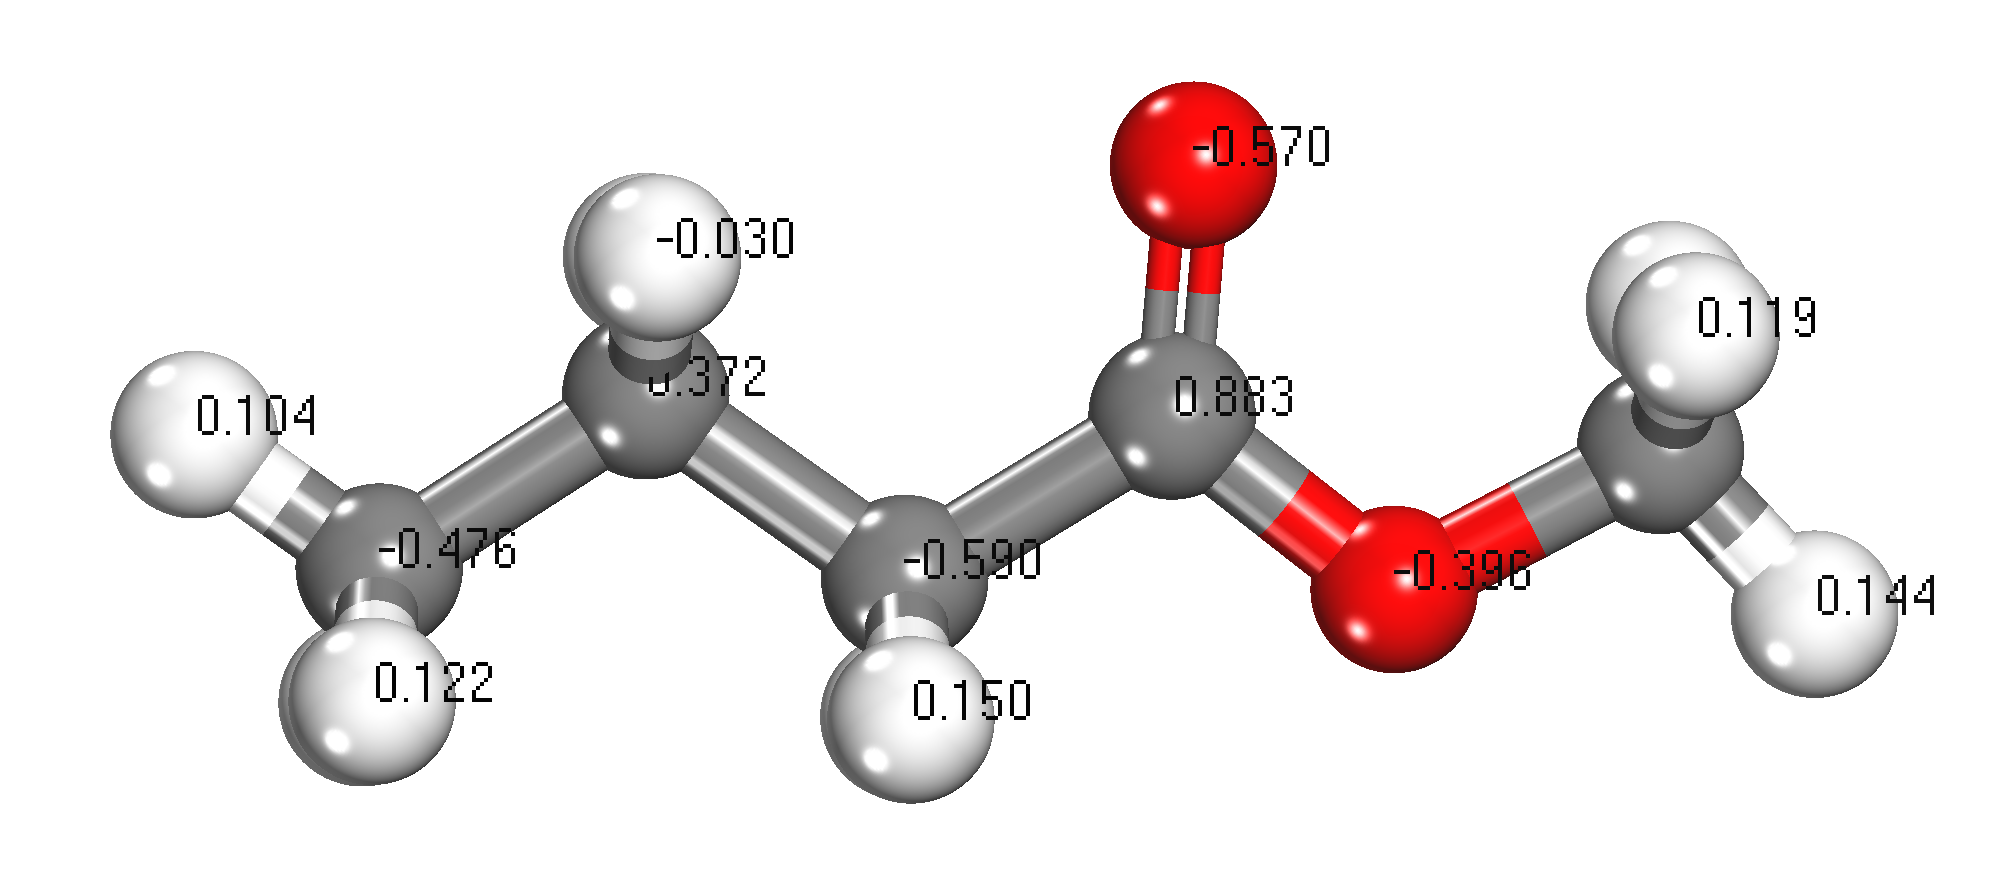
\includegraphics[width=0.6\textwidth]{figure/Building/saturatedC4.png}
%     \caption{丁酸甲酯模型电荷分布图}
%     \label{fig:sC4ESP}
% \end{figure}
% \subsubsection{丁烯酸甲酯模型结构}
% \par{优化后的丁酸甲酯分子模型的三维尺寸为1.732Å×7.757Å×2.755 Å,其具体三维结构见\reffig{fig:uC4ESP}。}
% \begin{figure}[H]
%     \centering
%     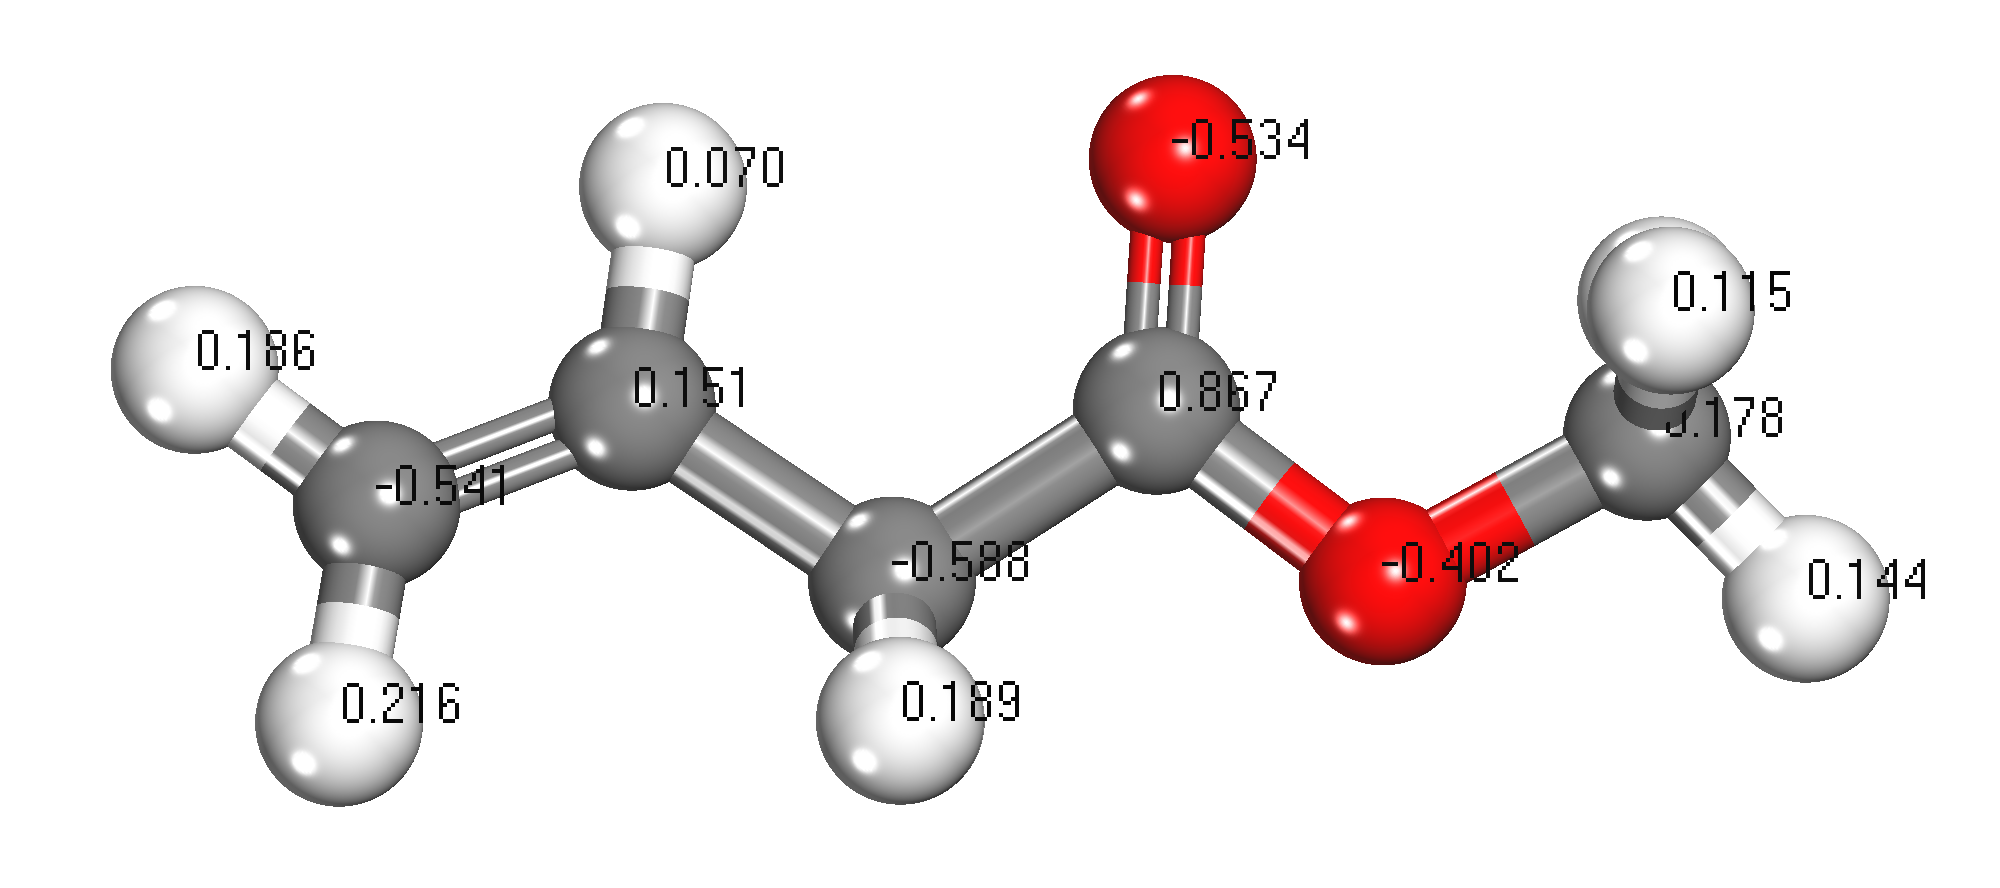
\includegraphics[width=0.6\textwidth]{figure/Building/unsaturatedC4.png}
%     \caption{丁烯酸甲酯模型电荷分布图}
%     \label{fig:uC4ESP}
% \end{figure}
% \subsubsection{乙酸甲酯模型结构}
% \par{优化后的乙酸甲酯分子模型的三维尺寸为1.732Å×5.228Å×2.755 Å,其具体三维结构见\reffig{fig:C2ESP}。}
% \begin{figure}[H]
%     \centering
%     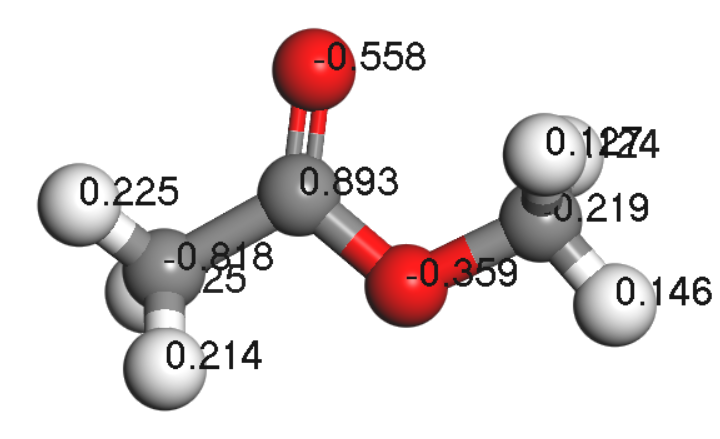
\includegraphics[width=0.5\textwidth]{figure/Building/C2.png}
%     \caption{乙酸甲酯模型电荷分布图}
%     \label{fig:C2ESP}
% \end{figure}
% \subsubsection{丙酸甲酯模型结构}
% \par{优化后的丙酸甲酯分子模型的三维尺寸为1.732Å×6.504Å×2.755 Å,其具体三维结构见\reffig{fig:C3ESP}。}
% \begin{figure}[H]
%     \centering
%     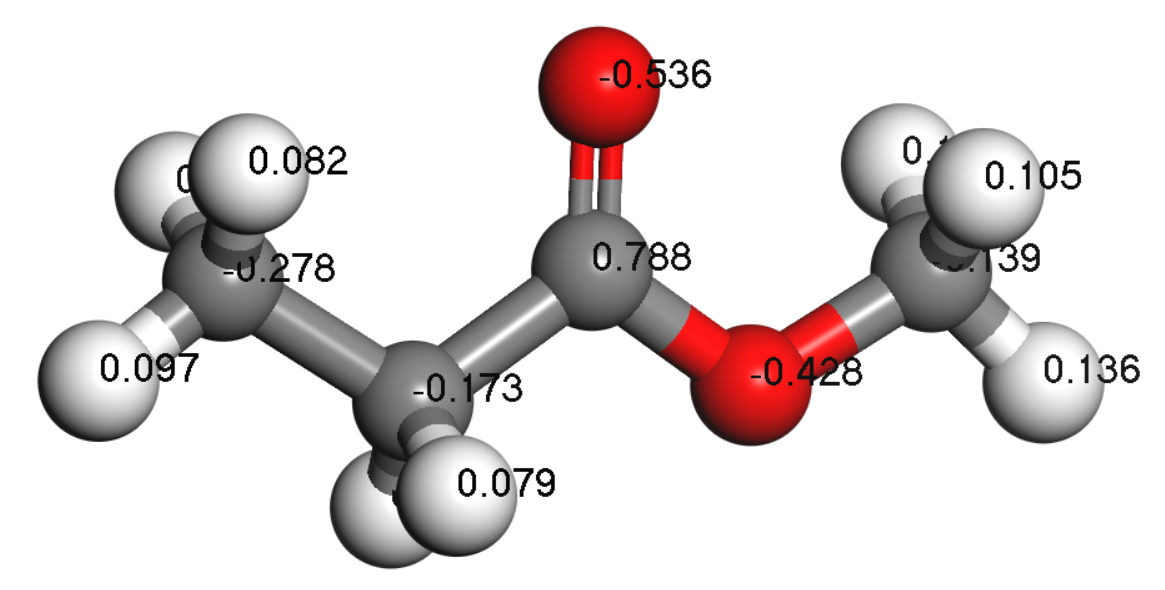
\includegraphics[width=0.6\textwidth]{figure/Building/C3.png}
%     \caption{丙酸甲酯模型电荷分布图}
%     \label{fig:C3ESP}
% \end{figure}
% \subsubsection{戊酸甲酯模型结构}
% \par{优化后的戊酸甲酯分子模型的三维尺寸为1.732Å×9.035Å×2.755 Å,其具体三维结构见\reffig{fig:C5ESP}。}
% \begin{figure}[H]
%     \centering
%     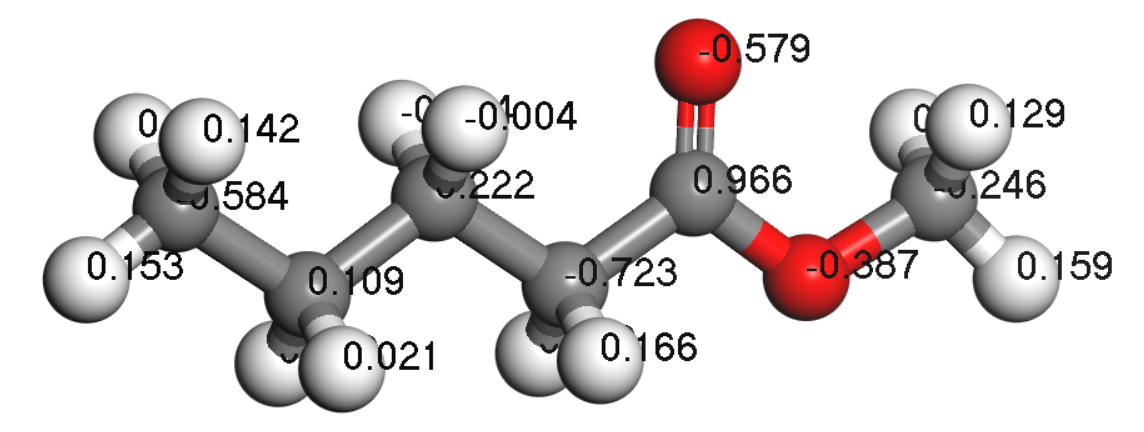
\includegraphics[width=0.6\textwidth]{figure/Building/C5.png}
%     \caption{戊酸甲酯模型电荷分布图}
%     \label{fig:C5ESP}
% \end{figure}
% \subsubsection{正己烷模型结构}
% \par{优化后的正己烷分子模型的三维尺寸为1.732Å×8.141Å×2.511 Å,其具体三维结构见\reffig{fig:C6ESP}。}
% \begin{figure}[H]
%     \centering
%     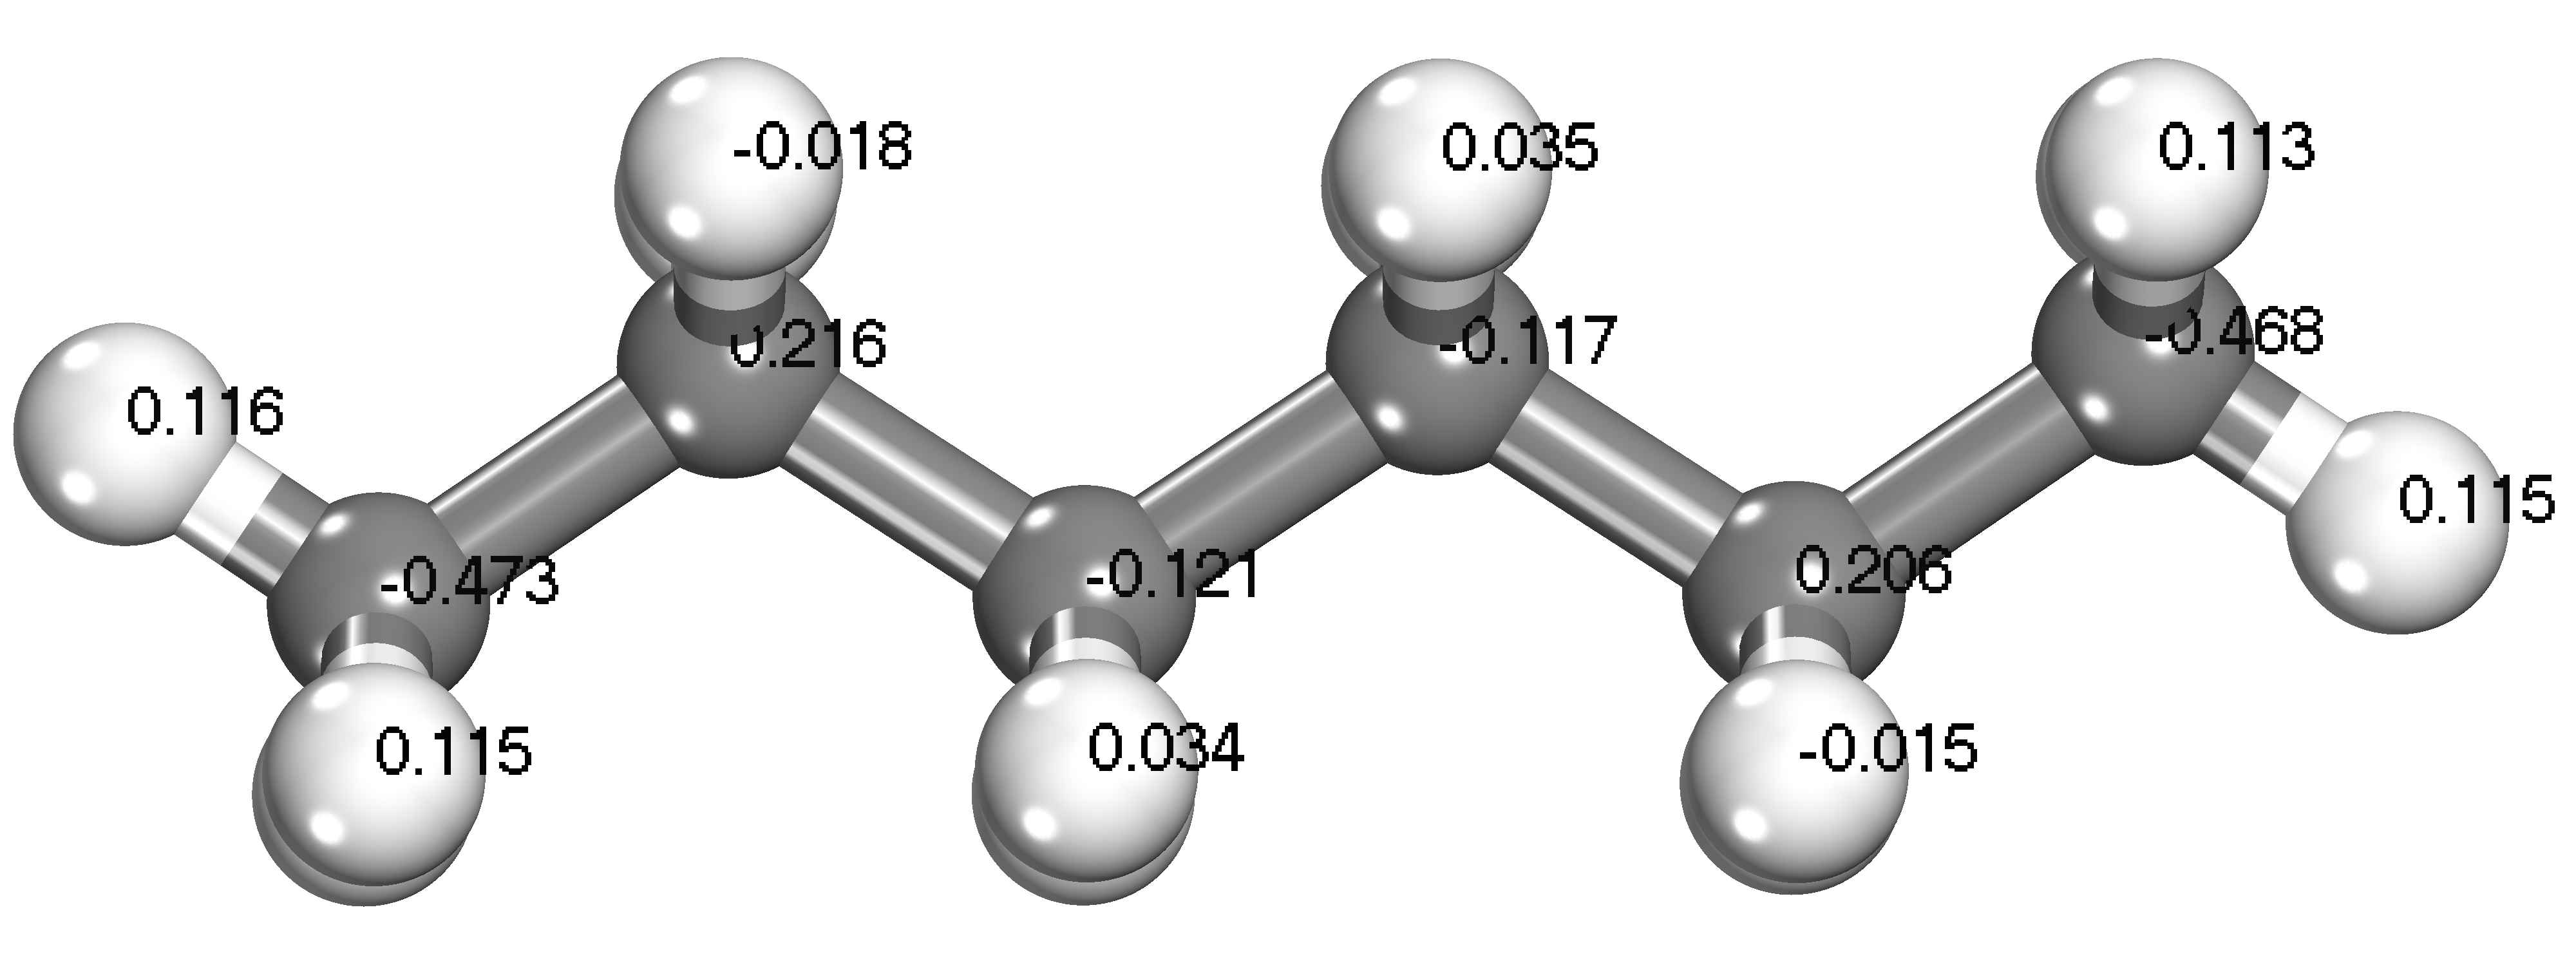
\includegraphics[width=0.6\textwidth]{figure/Building/C6.png}
%     \caption{正己烷模型电荷分布图}
%     \label{fig:C6ESP}
% \end{figure}
\subsection{H-ZSM-5微介孔分子筛模型构建与优化}
\subsubsection{Forcite 参数设置}\label{Forcite 参数设置}
\par{本节使用Forcite模块对H-ZSM-5分子筛进行结构优化以及确定各原子的电荷,相关参数设置如下:}
\begin{enumerate}
    \item 任务选择:结构优化(Geometry Optimization),收敛精度选择Ultra-Fine精度,算法选择默认的Smart方法;
    \item 力场(Forcefield)采用COMPASS\uppercase\expandafter{\romannumeral2}力场,其适用于大多数有机物、无机物、金属及其氧化物与卤化物,电荷选择Forcefield  assigned;
    \item 能量计算精度选择: Ultra-Fine精度;
    \item 加和方法(Summation method)中的静电相互作用(Electrostatic)选择埃瓦德方法(Ewald \& Group),非键相互作用(van der Waals)选择基于原子(Atom based)。
\end{enumerate}
% \par{一个合适的力场不仅能够计算出分子合理的最低构象,也能够准确地描述分子筛和吸附质分子之间的相互作用,所以力场选取的正确与否很大程度上决定了模拟结果是否可靠。本文选取的力场为COMPASS\uppercase\expandafter{\romannumeral2}。COMPASS\uppercase\expandafter{\romannumeral2}力场将 COMPASS 力场的应用范围扩大,可以用来预测聚合物和药物,并且修正了COMPASS力场的参数,使结果更加可靠\cite{Sun2016COMPASS}。而为了验证 COMPASS 力场的有效性,孙淮及其他研究者曾经对单个分子、液态分子及晶体分子共 28 类分子进行模拟验证\cite{分子模拟与高分子材料},发现COMPASS 力场能够模拟小分子与高分子,一些金属离子、金属氧化物与金属。}
\subsubsection{微孔模型构建及其优化}
\par{先导入MFI分子筛模型,其空间群为Pnma正交晶系结构。模拟采用2×2×3个晶胞\cite{bu2018diffusion},晶胞参数:a=40.044Å,b=39.798Å,c=40.149Å,α=β=γ=90°。首先根据文献\cite{danuthai2009conversion}的实验表征结果,将分子筛的硅铝比改为36,并根据文献\cite{zheng2014influence,zheng2016molecular}在Al原子相邻的O原子上引入H原子平衡电荷并作为反应活性位,并且H原子指向分子筛晶体中原有的骨架原子。最后使用Forcite模块进行结构优化和电荷赋值。}
\par{微孔H-ZSM-5分子筛超胞的分子式为:\ch{H_{31}O_{2304}Al_{31}Si_{1121}},有31个活性位,晶胞参数:a=40.044Å,b=39.798Å,c=40.149Å,α=β=γ=90°。其几何优化结构见\reffig{fig:mZSM},其中Si原子为黄色,Al原子为紫色,O原子为红色,H原子为白色。}
\begin{figure}[H]
    \centering

    \subfigure[A方向]{
    \begin{minipage}[t]{0.25\linewidth}
    \centering
    \includegraphics[width=1.5in]{figure/Building/microporeA.png}
    %\caption{fig1}
    \end{minipage}%
    }%
    \subfigure[B方向]{
    \begin{minipage}[t]{0.25\linewidth}
    \centering
    \includegraphics[width=1.5in]{figure/Building/microporeB.png}
    %\caption{fig2}
    \end{minipage}%
    }%
    \subfigure[C方向]{
    \begin{minipage}[t]{0.25\linewidth}
    \centering
    \includegraphics[width=1.5in]{figure/Building/microporeC.png}
    %\caption{fig2}
    \end{minipage}%
    }%
    \caption{微孔H-ZSM-5分子筛结构优化图}
    \label{fig:mZSM}
\end{figure}
\par{微孔分子筛经Forcite模块优化后,各原子之间的化学键方向发生了改变,H原子朝向也发生变化。模拟结果表明:微孔H-ZSM-5分子筛优化前体系能量为-78772.04 kcal/mol,优化后能量为-86248.41 kcal/mol;此时的分子筛能量最低,结构最稳定。}
\subsubsection{介孔模型构建及其优化}
\par{微孔H-ZSM-5 分子筛由沿B 方向的直通道和沿A 方向的锯齿形通道组成。在构建介孔模型时,选择沿C 方向的介孔来创建三维通道,以提高传质效率\cite{bu2018diffusion}。通过沿H-ZSM-5(4×4×3 单元)和(2×2×3 单元)两个超胞的C 方向切割,构建了60Å 和20Å 两种不同孔径的介孔H-ZSM-5 分子筛模型。两种介孔H-ZSM-5 分子筛模型的微孔壁厚度均为20Å,因此介孔体积分数分别为0.25和0.56。介孔表面硅原子以羟基封端。}
\par{20Å介孔H-ZSM-5分子筛超胞的分子式为:\ch{H_{171}O_{1800}Al_{27}Si_{837}},有27个活性位,晶胞参数:a=40.044Å,b=39.798Å,c=40.149Å。60Å介孔H-ZSM-5分子筛超胞的分子式为:\ch{H_{495}O_{4248}Al_{63}Si_{1953}},有63个活性位,晶胞参数:a=80.088Å,b=79.596Å,c=40.149Å。因为介孔A和B方向的结构和微孔的一样,所以只展示C方向的结构。介孔C方向的几何优化结构见\reffig{fig:2060ZSM},其中Si原子为黄色,Al原子为紫色,O原子为红色,H原子为白色。}
\begin{figure}[H]
    \centering

    \subfigure[20Å]{
    \begin{minipage}[t]{0.5\linewidth}
    \centering
    \includegraphics[width=3in]{figure/Building/20C.png}
    %\caption{fig1}
    \end{minipage}%
    }%
    \subfigure[60Å]{
    \begin{minipage}[t]{0.5\linewidth}
    \centering
    \includegraphics[width=3in]{figure/Building/60C.png}
    %\caption{fig2}
    \end{minipage}%
    }%
    \caption{介孔H-ZSM-5分子筛C方向结构优化图}
    \label{fig:2060ZSM}
\end{figure}

\subsubsection{分子筛中各原子电荷}
\par{优化后的分子筛中各原子电荷如\reftab{tab:ESP}所示。}

\begin{table}[H]
    \centering
    \caption{分子筛各原子所赋电荷表}
    \begin{tabular}{p{5cm}<{\centering}P{-1.3}}
        \toprule
        原子种类&\multicolumn{1}{p{5cm}<{\centering}}{电荷赋值}\\
        \midrule
        Si&1.400\\
        Al&0.800\\
        O&-0.700\\
        H&0.600\\
		\bottomrule
    \end{tabular}
	\label{tab:ESP}
\end{table}


\subsection{模型验证}
\par{为了验证所搭建的分子筛模型的结构是合理的,本文计算了结构优化后的微孔分子筛模型的X射线衍射图(XRD),并将结果和国际沸石协会(IZA-SC)数据库中的ZSM-5分子筛标准X射线衍射图\cite{baerlocher2007atlas}进行对比,结果如\reffig{fig:XRD}所示。从图中发现两者具有相同的特征峰,说明搭建的H-ZSM-5分子筛模型是合理的。}
\begin{figure}[H]
    \centering
    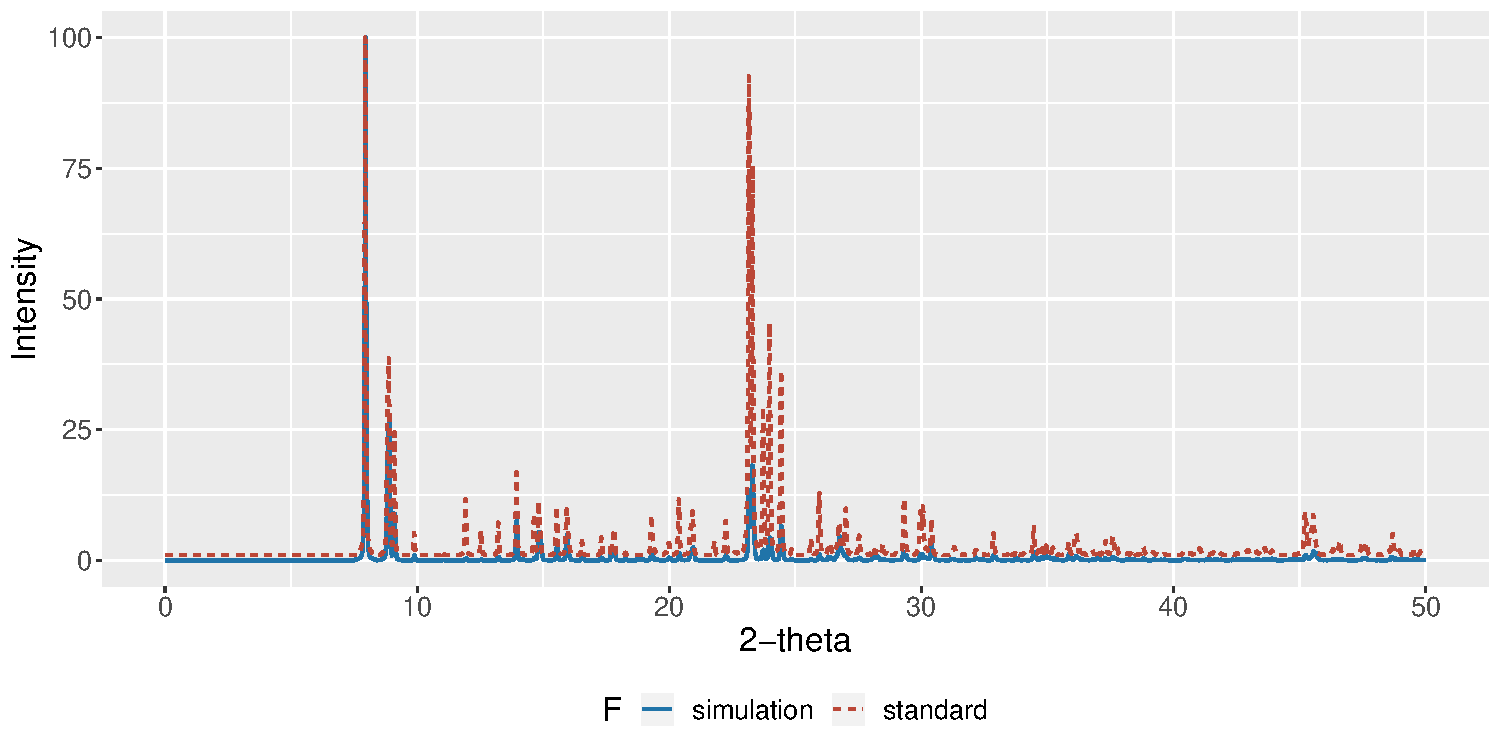
\includegraphics[height=0.5\textwidth]{figure/Building/XRD.pdf}
    \caption{微孔H-ZSM-5分子筛模型XRD与标准谱图对比图}
    \label{fig:XRD}
\end{figure}
\subsection{本章小结}
\par{本章通过Visualizer界面构建了丁酸甲酯、丁烯酸甲酯、油酸甲酯、反油酸甲酯和正己烷分子模型,并用Dmol3模块对进行其结构优化,并计算了ESP电荷,得到了吸附质分子的几何优化构型。}
\par{通过Visualizer界面构建了微介孔H-ZSM-5分子筛模型,并用Forcite模块对其进行结构优化,赋予电荷,得到了吸附剂分子的几何优化构型。}
\par{通过与标准X射线衍射图进行对比,验证了本文所构建的模型是合理的,为下文中吸附分子在H-ZSM-5分子筛中的吸附和扩散的模拟提供了合理的模拟基础。}
